\documentclass[12pt,twoside,a4paper]{article}


\usepackage[T1]{fontenc}
\usepackage[utf8]{inputenc}
\usepackage{graphicx}
\usepackage{RR}



%%%%%%%%%%%%%%%%%%%%%%%%%%%%%%%%%%%%%%%%%%%%%%%%%%%%%%%%%%%%%%%%%%%%%%%%%%%%%%%%
%%%                               80 COLONNES                                %%%
%%%%%%%%%%%%%%%%%%%%%%%%%%%%%%%%%%%%%%%%%%%%%%%%%%%%%%%%%%%%%%%%%%%%%%%%%%%%%%%%


%\RRNo{}

\RRetitle{A critical analysis of Contiki's network stack
          for integrating new MAC protocols}

\titlehead{A critical analysis of Contiki's network stack\ldots}

\RRauthor{
K\'evin Roussel
\and
Ye-Qiong Song
}

\RRequipe{Madynes}

\RRtitle{Analyse critique de la pile réseau de Contiki
         pour l'intégration de nouveaux protocoles MAC}

\RRabstract{
Recent Wireless Sensor Network (WSN) MAC protocols focus on both very low
idle traffic duty-cycle and high throughput when bursts of traffic occur.

It is highly desirable to be able to integrate them into a common and open
platform, not only for easing their performance comparison, but also
for their effective interaction with existing higher-layer protocols.

As part of our work on WSN, we have implemented a new Media Access Control
(MAC) protocol into the Contiki OS. When doing so, we stumbled into various
limitations and quirks, relative to this system---and especially
its network stack.

The present report summarizes the critical issues we have faced, and
gives some ideas to fix them or work around them. Considering the
widespread use of Contiki and its netstack, we believe that knowing
those issues will be helpful for other researchers and developers.
}

\RRkeyword{WSN, MAC protocols, Contiki OS, network stack}

\RRresume{
Les protocoles MAC récents pour réseaux de capteurs sans-fil (WSN) sont
conçus pour assurer à la fois une activité radio (``duty cycle'') minimale
durant les périodes d'inactivité sur le médium radio, et un débit maximal
quand des pointes de trafic réseau ont lieu.

Il est hautement préférable d'intégrer ces protocoles dans une plate-forme
commune et ouverte, non seulement pour faciliter la comparaison de leurs
performances, mais l'efficacité de leur interaction avec les protocoles
existants dand les couches supérieures de la pile réseau.

Durant nos travaux sur les WSN, nous avons implémenté un nouveau protocole
MAC (Media Access Control) au sein de Contiki OS. Ce faisant, nous avons
fait face à diverses limitations et difficultés techniques propres à ce
système~--- et notamment à sa pile réseau.

Le présent rapport résumé les problèmes critiques auxquels nous avons fait
face, et donne quelques idées pour les régler ou les contourner. Eu égard
à l'usage généralisé qui est fait de Contiki et de sa pile réseau, nous
pensons que de telles informations seront utiles aux autres chercheurs
et développeurs.
}

\RRmotcle{réseaux de capteurs sans-fil, protocoles MAC,
          Contiki OS, pile réseau}

\RRdate{December 2013}

\RCNancy


%%%%%%%%%%%%%%%%%%%%%%%%%%%%%%%%%%%%%%%%%%%%%%%%%%%%%%%%%%%%%%%%%%%%%%%%%%%%%%%%
%%%                               80 COLONNES                                %%%
%%%%%%%%%%%%%%%%%%%%%%%%%%%%%%%%%%%%%%%%%%%%%%%%%%%%%%%%%%%%%%%%%%%%%%%%%%%%%%%%

\begin{document}

\newcommand{\term}[1]{\textbf{#1}}

\makeRR


%%%%%%%%%%%%%%%%%%%%%%%%%%%%%%%%%%%%%%%%%%%%%%%%%%%%%%%%%%%%%%%%%%%%%%%%%%%%%

\section{Introduction}

Wireless Sensor Networks (WSNs) currently form a very active topic of
research. One aspect of this topic is the fast-paced development of
WSN-oriented operating systems.
Two projects clearly stand out in that domain: \term{TinyOS} \cite{tiny-os},
and \term{Contiki} \cite{contiki} \cite{contiki-web-site}.
Both are open-source projects, providing free\footnotemark{}
systems to the WSN-(and more generally embedded devices)-oriented community
of scientists and developers. We chose the latter as our software platform,
since it is written in standard C language (whereas TinyOS uses a specific
derivative named ``nesC''), and seems to be---as of now---more actively
used and supported by both scientific and industrial communities.

\footnotetext{Here, the term ``free'' is used as a synonym of liberty
              (of use and diffusion), as in the ``free speech'' expression.}

Another important aspect of WSN research is the optimization of
\term{Quality-of-Service (QoS)} and \term{energy consumption} directly into
the network stack mechanisms, especially at the \term{Media Access Control
(MAC)} level. This is an aspect on which many teams are actively working:
the standard \term{IEEE 802.15.4 MAC protocol} \cite{std802154}, with its
static, fixed duty-cycle, has been challenged by many other MAC protocols.
These alternative MAC protocols try to improve upon the standard by providing
dynamic runtime adaptation to the network traffic load, better QoS, and
minimized energy consumption (by allowing radio transceivers to be turned
off as much as possible); most of these alternatives are adaptive
duty-cycled protocols.

Adaptive duty-cycled protocols can be classified into many families:
some of the best-known protocols, like S-MAC \cite{s-mac} and
T-MAC \cite{t-mac}, are member of the synchronous MAC protocols family.
Others, like B-MAC \cite{b-mac}, X-MAC \cite{x-mac}, RI-MAC \cite{ri-mac},
and WiseMAC \cite{wise-mac} protocols, belong to the asynchronous MAC
protocols family. (Other families can be named, like frame-slotted,
or multichannel MAC protocols.) Among the asynchronous protocols,
we can distinguish between those based on the Low-Power Listening (LPL)
technique---such as B-MAC and X-MAC---and those using Low-Power
Probing (LPP)---like RI-MAC. The creator of the Contiki OS has himself
designed and published a MAC protocol, named ContikiMAC \cite{contiki-mac},
that is now the default protocol used by the Contiki OS. This protocol
is largely inspired from X-MAC and WiseMAC, and as such is also
an asynchronous, LPL-based, adaptive duty-cycled protocol.
Finally, ContikiMAC has itself served as a basis for further
improvements, notably the recent and promising
Strawman protocol \cite{strawman-mac}.

\begin{figure}[!t]
\centering
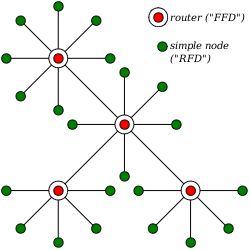
\includegraphics{star-topo-net.png}
\caption{An example of network using 2-tier, star-like topology.}
\label{star-topo-net}
\end{figure}
\hfil
\begin{figure}[!t]
\centering
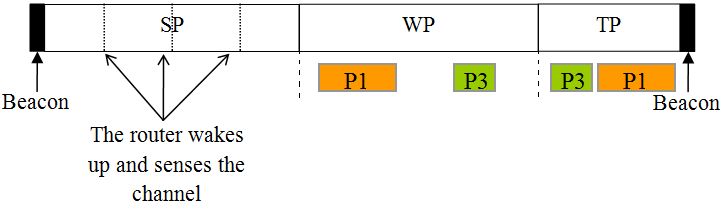
\includegraphics[width=11cm]{superframe.png}
\caption{The basic working principle of the CoSenS protocol.}
\label{cosens-principle}
\end{figure}

Our team is also active in this domain: we have already presented many
high performance traffic-adaptive MAC protocols for WSNs; among these stand
the \term{CoSens} \cite{cosens} protocol which has been implemented on
Jennic motes, and iQueue-MAC \cite{iqueue-mac} which has been implemented
on STM32W108 chips.

Although an actual implementation becomes nowadays almost a must step
to validate any new WSN MAC protocols, their specific implementation
does not allow a fair comparison. Worser, it is very hard to use them
within a full stack of protocols if routing or upper-layers are required.
So as already explained before, integrating those new protocols into
a well-accepted platform, such as Contiki, becomes highly desirable.

In this paper, we provide a critical analysis of important issues on
implementing new MAC protocols on Contiki network stack. This analysis
shows the limitations of actual version of Contiki and proposes improvements.

The simplicity of implementation has driven us to use CoSenS as a first
element of choice to implement into the Contiki network stack.
More evolved protocols, like iQueue-MAC, are planned to be implemented
in Contiki as soon as possible (as a second step).

Before detailing the issues we faced during this implementation work,
we will briefly summarize the workings of the CoSenS protocol.

%%%%%%%%%%%%%%%%%%%%%%%%%%%%%%%%%%%%%%%%%%%%%%%%%%%%%%%%%%%%%%%%%%%%%%%%%%%%%

\section{The CoSenS protocol: Quick Summary}

Since the CoSenS protocol is already explained and detailed in \cite{cosens},
we will here only quickly summarize its design and features, and thus explain
why we choose it as a first stepping stone in our exploration of Contiki's
internals.

CoSenS is designed for networks built upon a classical 2-tier, star-like
architecture (an example of which is represented on figure \ref{star-topo-net})
that can be, where one can distinguish between \term{router nodes}---that
can be assimilated to the ``Full-Function Devices'' (FFD) cited by
the 802.15.4 standard \cite{std802154}---and \term{simple, ``leaf''
nodes}---assimilable to 802.15.4 ``Reduced-Function Devices'' (RFD).
Simple nodes' role is mainly to perform measurements thanks to their
built-in sensors, and are supposed to possess only limited networking
abilities: they can only communicate with the router node they are
associated with---a simple node is always associated with one and only
one router that acts as its ``parent'' in the network. Conversely,
the routers run full-fledged network stacks, and are consequently
responsible for packet-routing duties through the network; thus,
each router act as a gateway for a variable number of simple nodes,
that are designated as the router's ``children''.

CoSenS is designed to run on the router nodes, while the simple nodes
are supposed to use the classical CSMA/CA protocol. They are always
in sleeping mode unless they have packets to send.
CoSenS is derived from that classical CSMA/CA protocol, improving
significantly on it in terms of performance for medium and high traffic
loads, and thus facilitating the implementation of QoS mechanisms.

The basic idea of CoSenS is the following: the duty cycle of a router node
is divided into three periods: a \term{Sleep Period (SP)} where the router
goes to sleep but periodically wakes up and senses the channel to receive
its neighboring router's packets, a reception period where the router
passively waits for packets to be received---this period is thus named
\term{Waiting Period (WP)}---, and a \term{Transmission Period (TP)}, during
which it will transmit the packets it received. Indeed, when a router
receives a packet (during a WP), it won't retransmit it right away;
that packet will be enqueued, for deferred retransmission during
the next TP. During these TPs, enqueued packets are sent in ``burst-mode'',
avoiding the overhead related to the channel acquisition procedure of the
CSMA/CA protocol for all but the first sent packet (which will use CSMA/CA,
followed by a preamble similar to that of B-MAC). Routers' duty cycles,
under CoSenS, simply consist in the succession of SPs (sleep for saving
energy), WPs (for receiving packets) and TPs (for retransmitting them).

That simple mechanism (a ``Sleep, Collect then Send burst scheme'', as its
author calls it) that can be summarized by figure \ref{cosens-principle},
gives nevertheless a significant performance advantage to CoSenS over
both the standard 802.15.4 MAC and the classical CSMA/CA protocols.
Moreover, its simplicity of design and implementation has naturally
driven us to choose it as the first protocol we would try to implement,
as a beginning of our work into Contiki's network stack.

%%%%%%%%%%%%%%%%%%%%%%%%%%%%%%%%%%%%%%%%%%%%%%%%%%%%%%%%%%%%%%%%%%%%%%%%%%%%%

\section{Working with the Contiki Network Stack}

While implementing the CoSenS protocol as an addition to the Contiki's
network stack (\term{``netstack''}), we discovered many issues that
hinder development into Contiki, both in general and at the specific level
of the netstack. We will now detail these issues, and---when possible---make
propositions to fix or at least work around these problems.

%%%%%%%%%%%%%%%%%%%%%%%%%%%%%%%%%%%%%%%%%%%%%%%%%%%%%%%%%%%%%%%%%%%%%%%%%%%%%

\subsection{Lack of documentation}

This is a recurrent problem with Contiki: apart from source code comments
and examples, there is actually almost no documentation. This concerns
all of Contiki in general, and as such its netstack in particular.

One can especially point the total absence of technical reference documents,
where the general architecture of the system, as well as design and
implementation choices, could be explained; such reference documents
quickly become key tools to really understand a software platform,
and thus to be able to become a proficient developer.

There is also a serious shortage on tutorials: the only official introductory
document is the ``get started'' web page, that will quickly show you how to
use the provided ``Instant Contiki'' Linux distribution to start simulations
(using the project's simulator named \term{Cooja} \cite{cooja}) and download
program examples to hardware. No document will teach you and (more
importantly) explain you the various features of the Cooja simulator,
no document will show you how to program applications on Contiki, what are
the specificities of embedded development (when compared to ``classical''
programming for PCs)---even less how to touch its internals!
Such absence makes the initial approach to Contiki for new developers
difficult, by further heightening an already high learning barrier.

The main source of documentation, when it comes to Contiki development,
is the ``contiki-developers'' mailing list \cite{contiki-dev-ml}: any person
wishing to do development on this platform (be it at the applicative or at
the system level) just won't be able to achieve any real goal without
subscribing to it, and requesting informations and help from its members.
While this list provides a rich source of knowledge, is reactive, and
friendly welcomes newcomers, it can hardly be considered as a satisfactory
replacement for the missing technical and introductory documentation
mentioned above.

Let's also add that, if there are many examples provided of application-level
code using Contiki OS, there is no such examples of code working at the
system-level (i.e.: designed to plug into Contiki's internals). This kind
of development is thus even more difficult to apprehend and learn.

%%%%%%%%%%%%%%%%%%%%%%%%%%%%%%%%%%%%%%%%%%%%%%%%%%%%%%%%%%%%%%%%%%%%%%%%%%%%%

\subsection{Limitations}

Many limitations found in Contiki were dicted by the constraints imposed
by the devices that constitute WSNs: they are indeed very limited when
it comes to processing power and (especially) memory space.

Nevertheless, one of them is just a ``missed point'' that can be completed
quite easily with some additional code.

We will begin the following list with this missing element, then examine
deeper problems, that are the direct consequences of some basic design
choices made for the Contiki netstack.

%%%%%%%%%%%%%%%%%%%%%%%%%%%%%%%%%%%%%%%%%%%%%%%%%%%%%%%%%%%%%%%%%%%%%%%%%%%%%

\subsubsection{Missing features: incomplete radio drivers}

As of the current version (release 2.7), the API for the radio transceivers
drivers only provides the most basic features: sending and receiving
a packet, turning transceiver on and off, and checking for channel
availability (CCA). Access to all other features of transceivers (e.g.:
frequency/channel switching, transmission power setting, changing node
address(es), etc.) forces to directly access the transceiver, thus breaking
portability and separation between netstack layers.

To solve this problem, we have submitted an API extension, allowing
to access these extended features via a standard and flexible "capabilities"
mechanism, without breaking compatibility with existing code, and incurring
only minimal overhead (addition of three mere pointers to a radio driver
definition). The three added function pointers serve respectively to
1)~query the radio transceiver for built-in configuration constants
(e.g.: maximal power level for packet emission), 2)~to get and
3)~to set configuration parameters---a.k.a. ``capabilities''---impacting
the behaviour of the radio transceiver (e.g.: radio channel,
node address(es), etc.). We are currently waiting for the
response of the project's maintainers to our contribution.

%%%%%%%%%%%%%%%%%%%%%%%%%%%%%%%%%%%%%%%%%%%%%%%%%%%%%%%%%%%%%%%%%%%%%%%%%%%%%

\subsubsection{Netstack centered on an unique ``packetbuf''}

One very specific feature of Contiki's netstack is that it is centered
around a unique packet buffer (named \term{``packetbuf''}), that constitutes
the mandatory ``work area'' for the various netstack layers (see below).

This design pattern was chosen to spare precious memory: on wireless sensor
devices, program code must indeed fit in dozens of kilobytes of flash RAM,
while data---and among them, network packets---is restricted to very
limitative amounts of RAM (sometimes nothing more than 2 kilobytes!).

Unfortunately, this design choice has some undesirable consequences:
\begin{itemize}
\item packet loss: since that unique buffer is to be used by \emph{all
      and every part of the netstack, at every time}, any breach in
      the synchronization between the various netstack components
      may result in overwriting the ``packetbuf'' at the wrong time,
      thus provoking data loss! The risk of a packet incoming (i.e. being
      received by the radio transceiver) during the processing of another
      data by the netstack, is especially critical, since the arrival of
      external data is, by nature, an event that code (even at
      system-level) cannot plan nor avoid.
\item unabilty to handle queues efficiently: designing efficient MAC protocols
      almost always implies to handle packet queues (both in emission and
      reception); while Contiki also provides mechanisms for them
      (``queuebuf'', ``packetqueue''), the unique ``packetbuf''-centered
      design means unceasing copies between that ``packetbuf'' and the queues,
      that is: waste of time, processing power, and even memory---being
      able to designate a portion of memory (i.e.: a given packet in a
      queue) as the current work area at runtime would actually use less
      memory than the current ``unique packetbuf'' scheme. Also note that
      the provided ``queuebuf'' and ``packetqueue'' mechanisms have themselves
      a complex and counter-intuitive design and use, because they need to
      work with the unique ``packetbuf''.
\item netstack complexity: the need to handle correctly that unique packet
      buffer actually contributes to make the netstack code more complex,
      since the various elements of the netstack need to perform various
      operations that can become quite complex---like careful synchronization,
      or never-ceasing copies to/from packet queues---that wouldn't be
      needed on a more flexible (e.g.: queue-based) design.
\end{itemize}

\begin{figure}[!t]
\centering
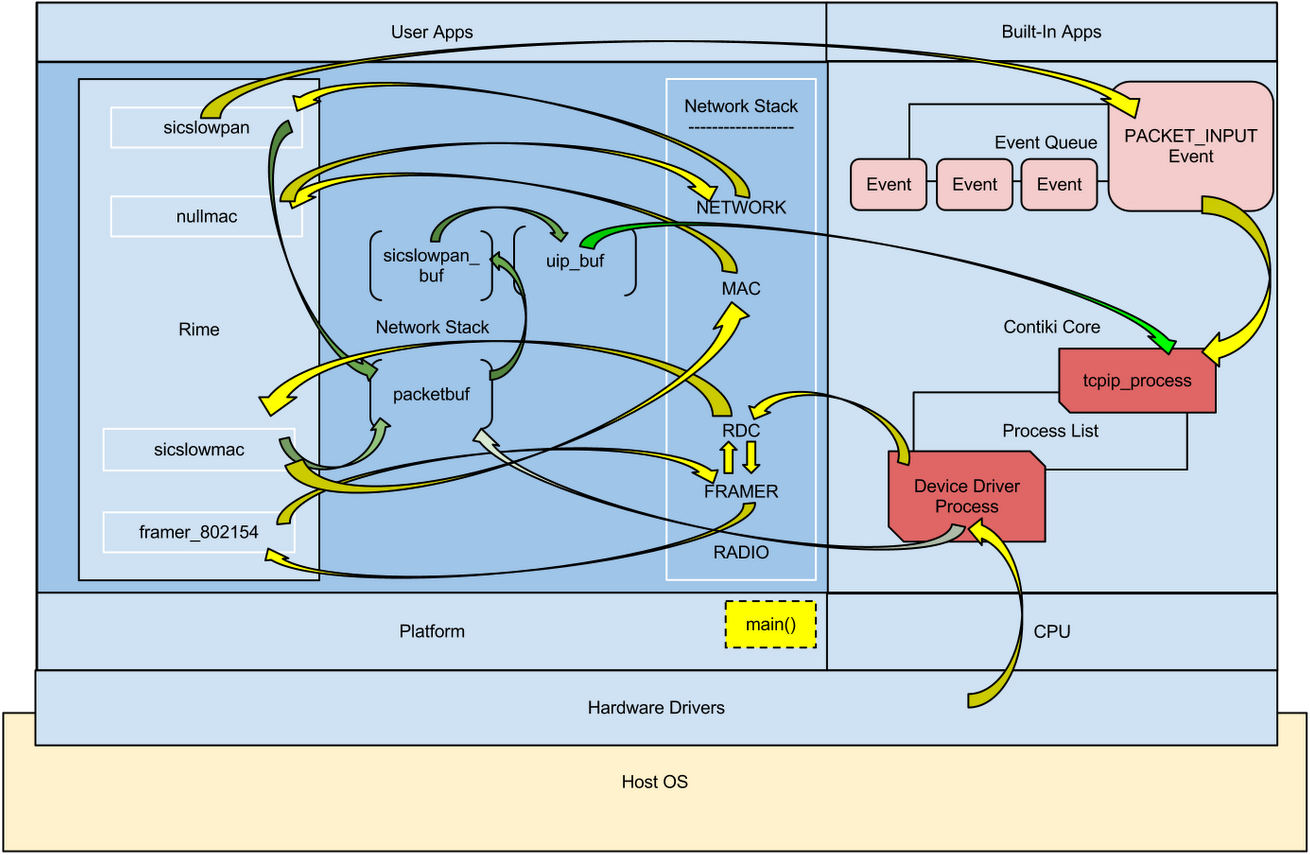
\includegraphics[width=13.5cm]{ContikiNetstack.png}
\caption{Functional representation of Contiki netstack's layered architecture
         (from \cite{judit-blog}).}
\label{contiki-netstack}
\vskip 5mm plus 5mm minus 4mm
\end{figure}

%%%%%%%%%%%%%%%%%%%%%%%%%%%%%%%%%%%%%%%%%%%%%%%%%%%%%%%%%%%%%%%%%%%%%%%%%%%%%

\subsubsection{Separation of MAC and RDC layers}

The Contiki netstack is designed around the principle of layer separation.
There are indeed distinct drivers for radio transceivers, routing protocols,
etc.

As a part of this strategy, there is a distinction, in Contiki, between
the \term{Radio Duty Cycle (RDC)} layer---that is supposed to control
how the radio transceiver is turned on and off during duty cycles, thus
implementing the energy-saving strategy---and the \term{Media Access
Control (MAC)} layer---that is (theoretically) only tasked with
ordering and sequencing packet transmissions.

In practice, most modern MAC protocols do manage both of these aspects,
in order to adapt dynamically network efficiency (QoS) \emph{and} energy
consumption to the ongoing traffic (e.g.: \cite{x-mac} \cite{ri-mac}
\cite{cosens} \cite{iqueue-mac}, among others). This separation consequently
becomes artificial, and only adds more unneeded complexity to MAC protocol
implementations, since separating these two aspects is at best difficult,
and often impossible: as an example, the ContikiMAC protocol is itself
implemented as a sole RDC driver (preferably used with a ``null'' MAC
driver).

%%%%%%%%%%%%%%%%%%%%%%%%%%%%%%%%%%%%%%%%%%%%%%%%%%%%%%%%%%%%%%%%%%%%%%%%%%%%%

\subsubsection{Excessive complexity of the netstack}

As a generalization of the previous point, most of the Contiki netstack
suffers from excessive ``layerization'': there is indeed no less than five
levels involved (from bottom to top):
\begin{enumerate}
\item RADIO: the ``physical'' driver controlling the radio transceiver;
\item FRAMER: the parser/generator of formatted packets (e.g.:
              ``\texttt{framer\_ 802154}'' for the 802.15.4 protocol);
\item RDC: the Radio Duty-Cycle controller (see above);
\item MAC: the Media Acess Control protocol implementation;
\item NETWORK: the network-level protocol implementation (e.g. 6LoWPAN).
\end{enumerate}

If such a design can (in theory) provide more flexibility in the
implementation, it actually add its complexity to the other
constraints of the netstack: namely, the unique ``packetbuf'' architecture,
the difficulty to clearly separate between layers (see the previous point),
the need to interact smoothly with other parts of the system---especially
the event and the protothread \cite{pt} subsystems, that allow Contiki
to offer lightweight cooperative multitasking features.

The layered architecture of Contiki network stack can be summarized
by figure \ref{contiki-netstack} (from \cite{judit-blog});
one can easily see on this figure the complexity induced by
the netstack's design choices.

Combined with the lack of available documentation (especially technical
references), this all makes contributing code to that netstack a difficult,
tedious, and error-prone task.

Moreover, since these difficulties are direct consequences of netstack's
fundamental design principles, fixing them is not envisionable without
reworking most of the system's internals, which would imply major (and
most likely unacceptable) compatibility breaks for the system-level code.
The need for a precise, helpful, detailed technical documentation is thus
even more critical.

%%%%%%%%%%%%%%%%%%%%%%%%%%%%%%%%%%%%%%%%%%%%%%%%%%%%%%%%%%%%%%%%%%%%%%%%%%%%%

\section{Conclusion}

We have summarized, in the present paper, the issues we had to face when
trying to implement a new MAC protocol into Contiki's network stack;
these issues---especially the lack of technical documentation---are
most likely to be encountered by every developer undertaking the
development of system-level code into Contiki OS (and probably
even, at a lesser degree, development of application-level code).

As a attempt to bring solutions to these problems, we have taken
different actions: we have proposed code contributions designed
to add missing features (especially at the radio drivers level);
and we have identified some problematic points that developers
are bound to meet, thus paving the way towards a comprehensive
set of technical documentation and tutorials we wish to contribute,
at a later point, to the Contiki project.

Thus, we hope, by facilitating the task of developers, to contribute
to widen even further the diffusion and use of the Contiki, as we
believe that this OS has not only already proven to be a very
valuable asset to the WSN research and development community, but also
has still much to offer.

%%%%%%%%%%%%%%%%%%%%%%%%%%%%%%%%%%%%%%%%%%%%%%%%%%%%%%%%%%%%%%%%%%%%%%%%%%%%%

\section*{Acknowledgment}

The authors would like to thank the \emph{Living Assistant Robot}
and the \emph{ANR Quasimodo} (ANR grant \#~2010 INTB 0206 01) projects,
for providing fundings to the research work corresponding
to the present paper.



\bibliographystyle{IEEEtran}
{\small
\bibliography{analysis-contiki-netstack}}

\end{document}
